\section{Struttura Programma Java}
Un programma Java è composta da librerie di classi del JDK, Package\footnote{Contenitori, gerarcici tra loro, di una decina di classi di alto livello con scopo comune.} e Moduli\footnote{Insieme di Package costituente un frammento di codice autonomo.}, librerie di esterne e un insieme di classi fondamentali.

La classe cardine di un programma è la class main\footnote{Un main è il punto d'accesso di un programma.}.
\multiline{main}{}{CodiciEsempio/main.java}
Il parametro del main è un array di stringhe che sono i parametri che l'utente può immettere da tastiera quando il programma è lanciato da CLI. Poco usato.

\subsection{Esecuzione Programma}
\begin{enumerate}
	\item Salvare la classe in un file \textbf{"NomeClasse.java"}.
	\item Compilare con \textit{javac NomeFileClasse.java}. Genererà il \textbf{bytecode NomeFileClasse.class} per la JVM.
	\item Esegiure con \textit{java NomeFileClasse}. La JVM cercherà il main da cui partire a eseguire.
\end{enumerate}
Lavorando con più file: si compila tutto con \textit{javac *.java} poi si esegue solo il bytecode contenente la classe main.

\subsection{I package}
Per prassi nella cartella di un progetto, si fa corrispondere hai package auto-costruiti delle directory del file system.

Di default il package di una unità di compilazione\footnote{File.java compilabile atomicamente contenente classi una dopo l'altra.}, ".java", è la root di gerarchia.
Per definire il pakage di appartenenza si specifica a inizio sorgente:

\inline{package <pName>;}

Per poi usare una classe di un package bisogna importarla (non aggiunge codice nell'eseguibile):
\begin{itemize}
	\item \inline{import java...;} importa una singola classe.
	\item \inline{import java...*;} importa l'intero Package.
	\item \inline{import java.lang.*;} importazione di default.
\end{itemize}
Il nome completo di una classe dipende dal Package in cui si trova. Se non si importa bisogna specificare all'uso il nome completo.

\subsubsection{Compilazione ed'esecuzione Avanzata}
Per tenere sorgenti e eseguibili separati, in progetti grandi si dispone la cartella \textit{src} per i sorgenti (.java) e la cartella \textit{bin} per i bytecode (.class).

\oneline{javac -d "<dirExe>" [-cp "<lib1:|;...>"] <.../elencoSorgenti>}

\oneline{java -cp "<dirExe[lib1:|;...]>" <fullyClasseMain>}

\begin{itemize}
	\item \inline{-d} specifica al compilatore la cartella dove creare i .class. Se non già presente la crea.
	\item \inline{-cp} linka le classi dei percorsi specificati (divisi da : o ;) al classpath\footnote{Sottopercorso (insieme ordinato) di cartelle che corrisponde al percorso del package dichiarato per la classe corrispondente. Il classpath di default è il JRE (Java Runtime Environment).}.
	\item La JVM si aspetta il FQCN (Fully-Qualified Class Name).
\end{itemize}

\subsubsection{Gradle}
Build system ibrido composto da:
\begin{itemize}
	\item \textbf{Progetto} Cartella contenente i file \textit{build.gradle.kts} e/o \textit{settings.gradle.kts} (build files).
	\begin{enumerate}
		\item Il build contiene la logica di costruzione del software.

		\oneline{plugins\{java\}}

		Io creo \textit{src/main/java} per i .java e sarà creato \textit{build/classes/java/main} per i .class.
		\item Il settings contine la personalizzazione, come il nome del progetto.

		\oneline{rootProject.name="..."}
	\end{enumerate}
	\item \textbf{Plugin} Sofware contenente \textit{task} pronti all'uso, come per java.
	\item \textbf{Task} Singola operazione atomica del processo di costrutzione del software. Una esecuzione gradle richiede una o più task di cui sono automaticamente dedotte le dipendenze.

	Comandi: gradle tasks, gradle tasks --all, gradle compileJava, gradle clean.
\end{itemize}
L'esecuzione è delegata al compilatore del linguaggio specifico.

\textbf{Wrapper}: sofware scarica gradle e lo usa per creare il sofware.
File del wrapper: gradle/wrapper/gradle-wrapper.jar (wrapper in s'è), gradle/wrapper/gradle-wrapper.properties (versione), ./gradlew oppure gradlew.bat (eseguono il wrapper).

Per compilare:
\oneline{./gradlew compileJava}

\subsubsection{Analisi Statica}
Tramite \textbf{Sofware di analisi statica del codice} si corregge, migliora e uniforma stilisticamente il codice (auto per controllo versione).
Modalità: Stand-alone, plug-in, plugin Gradle.

La modalità \textbf{plugin Gradle} si compone di: SpotBugs, PMD e CPM, Checkstyle. Si configura in \inline{build.gradle.kts} con:

\oneline{plugins \{ id("org.danilopianini.gradle-java-qa") version "1.75.0"\}}

Falsi positivi/negativi si gestisce attuando la \textbf{sospensione} dello strumento:
\begin{itemize}
	\item \textbf{SpotBugs} si sospende con l'annotazione \inline{@SuppressFBWarnings(...)} della libreria che si include in \inline{build.gradle.kts}:

	\oneline{dependencies \{ compileOnly("com.github.spotbugs:spotbugs-annotations:4.7.3") \}}

	\item \textbf{PMD} si sospende con un commento in linea.

	\oneline{... // NOPMD [spiegazione sospensione]}

	\item \textbf{Checkstyle} si sospende una regola specifica.

	\multiline{}{}{CodiciEsempio/checkstyle.java}
\end{itemize}

\subsubsection{Uso librerie esterne}
Per far scaricare, salvare nella home user directory, includere nel classpath a Gradle bisogna:
\begin{enumerate}
	\item Configurare in \inline{build.gradle.kts: repositories \{mavenCentral()\}}.

	\item Indicare in \inline{build.gradle.kts: dependencies \{"scope(libStandardName)" ...\}}.

	scope: \inline{implementation, testImplementation, testRunTimeOnly}.
\end{enumerate}

\subsubsection{Struttura gradle}
\begin{center}
	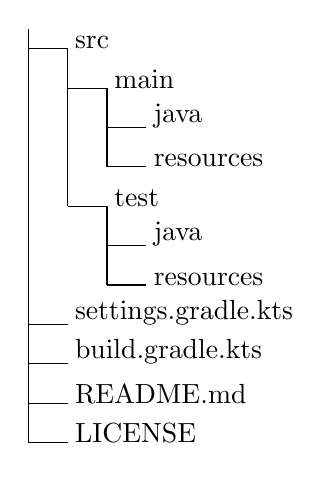
\begin{tikzpicture}[scale=0.5]
		\node[black, anchor=south west] at (-2.06,0.25) {src};
		\node[black, anchor=south west] at (-0.06,-1.75) {java};
		\node[black, anchor=south west] at (-0.06,-2.75) {resources};
		\node[black, anchor=south west] at (-1.06,-3.75) {test};
		\node[black, anchor=south west] at (-0.06,-4.75) {java};
		\node[black, anchor=south west] at (-0.06,-5.75) {resources};
		\node[black, anchor=south west] at (-2.06,-7.75) {build.gradle.kts};
		\node[black, anchor=south west] at (-2.06,-6.75) {settings.gradle.kts};
		\node[black, anchor=south west] at (-2.06,-9.75) {LICENSE};
		\node[black, anchor=south west] at (-2.06,-8.75) {README.md};
		\node[black, anchor=south west] at (-1.06,-0.75) {main};
		\draw[draw=black, thin, solid] (-2.00,-6.50) -- (-3.00,-6.50);
		\draw[draw=black, thin, solid] (-2.00,-7.50) -- (-3.00,-7.50);
		\draw[draw=black, thin, solid] (-2.00,-8.50) -- (-3.00,-8.50);
		\draw[draw=black, thin, solid] (-2.00,-9.50) -- (-3.00,-9.50);
		\draw[draw=black, thin, solid] (-2.00,0.50) -- (-3.00,0.50);
		\draw[draw=black, thin, solid] (-3.00,-9.50) -- (-3.00,1.00);
		\draw[draw=black, thin, solid] (-2.00,0.50) -- (-2.00,-3.50);
		\draw[draw=black, thin, solid] (-2.00,-3.50) -- (-1.00,-3.50);
		\draw[draw=black, thin, solid] (-2.00,-0.50) -- (-1.00,-0.50);
		\draw[draw=black, thin, solid] (-1.00,-0.50) -- (-1.00,-2.50);
		\draw[draw=black, thin, solid] (-1.00,-1.50) -- (0.00,-1.50);
		\draw[draw=black, thin, solid] (-1.00,-2.50) -- (0.00,-2.50);
		\draw[draw=black, thin, solid] (-1.00,-3.50) -- (-1.00,-5.50);
		\draw[draw=black, thin, solid] (-1.00,-5.50) -- (0.00,-5.50);
		\draw[draw=black, thin, solid] (-1.00,-4.50) -- (0.00,-4.50);
	\end{tikzpicture}
\end{center}

\begin{itemize}
	\item Per risorse s'intende tutto tranne librerie o sorgenti.
	\item \inline{README.md} contiene descrizione, autori, guida all'uso, link, risorse.
	\item \inline{LICENSE} per un progetto open source come MIT o similari.
\end{itemize}

\subsection{Convenzioni}
\begin{itemize}
	\item Linee max 90 caratteri e indenzazione 2-4 caratteri.
	\item Una sola istruzione per riga e quindi si definisce una sola variabile per riga, quando necessario, sempre inizializzata.
	\item Apertura "\{" a fine riga della dichiarazione e chiusura "\}" in linea a dove inizia la riga di apertura.
	\item Condice senza righe vuote di separazione a meno di metodi/costruttori.
	\item Non usare assegnamenti dentro espressioni e usare parentesi solo in espressioni non banali.
	\item Nomi classi e interfacce in "PascalCase". Nomi metodi, campi, variabili in "camelCase" e costanti in "SNAKE\_CASE". Nomi di package in minuscolo con numeri e senza "\_".
	\bigskip
	\item I metodi che returnano, senza parametri, si chiamano \inline{get...} oppure \inline{is/has...} se return boolean.
	\item I metodi che returnano void, e accettano parametri, si chiamano \inline{set...}.
\end{itemize}